\documentclass[a4paper,10pt]{article}
\usepackage[utf8]{inputenc}
\usepackage[margin=1.5cm]{geometry}
\usepackage{amsmath}
\usepackage{listings}
\usepackage{tikz}
\usepackage{siunitx}
\usepackage{pgfplots}
\usepackage{hyperref}
\usepgfplotslibrary{units} % Allows to enter the units nicely

\title{Codegeneratoren}
\author{Sebastian Geiger\\ \small{Twitter: @lanoxx, Email: sbastig@gmx.net}}

\lstset{ %
  %backgroundcolor=\color{background},   % choose the background color; you must add \usepackage{color} or \usepackage{xcolor}
  basicstyle=\small\ttfamily,        % the size of the fonts that are used for the code
  %commentstyle=\color{mygreen},    % comment style
  %frame=lines,                    % adds a frame around the code
  columns=fixed,
  %keywordstyle=\color{blue},       % keyword style
  language=Java,                 % the language of the code
  numbers=left,                    % where to put the line-numbers; possible values are (none, left, right)
  numbersep=5pt,                   % how far the line-numbers are from the code
  %numberstyle=\scriptsize\color{mygray}, % the style that is used for the line-numbers
  showspaces=false,                % show spaces everywhere adding particular underscores; it overrides 'showstringspaces'
  showstringspaces=false,          % underline spaces within strings only
  showtabs=false,                  % show tabs within strings adding particular underscores
  %stringstyle=\color{mymauve},     % string literal style
  tabsize=2                       % sets default tabsize to 2 spaces
}


\sisetup{
  round-mode          = places,
  round-precision     = 2,
}

\begin{document}

\maketitle

\begin{abstract}
This is a very short summary of the topics that are tought in ``Codegeneratoren``. Code generators are the backend part of a compiler 
that deal with the conversion of the machine independent intermediate representation into machine dependent instructions and the various 
optimizations on the resulting code. The first two Sections deal with prerequisits that are required for the later parts. Section 1 
discusses \textit{computer architectures} in order to give a better understanding of how processors work and why different optimizations 
are possible. Section 2 discusses some of the higher level \textit{optimizations} that are done before the code generator does its work. 
Section 3 discusses \textit{instruction selection}, which conserns the actual conversion of the intermediate representation into machine 
dependent instructions. The later chapters all deal with different kinds of optimizations that are possible on the resulting code.

I have written this document to help my self studing for this subject. If you find this document useful or if you find errors or mistakes 
then please send me an email.
\end{abstract}

\tableofcontents

\section{Computer architectures}
Codegenerators are dependent on the computer architecture they are designed for. Therefore a comprehensive understanding of the different 
concepts of computer architectures is requried. This capter can be roughly split into two main aspects: \textbf{microarchitectures} and 
\textbf{Instruction Set Architectures} sometimes abbreviated ISA. The concept of \textit{microarchitectures} referes to the hardware part 
of a processor, that is its different parts such as execution units, pipelines, caches and such. The instruction set architecture defines 
the interface between the processor and its users (usually assembler programmers or compiler writers). It is easy to see that a 
codegenerator is dependent on the instruction set architecture it was designed for. For example a different codegenerator is needed for 
CISC and RISC computers. But a codegenerator developer also needs a good understanding of the underlying microarchitecture in order to 
better optimize the generated code. An example for such optimizations is the use of instruction level parallelism or code scheduling to 
achieve a higher pipeline utilization. Below the most important concepts of microarchitectures and ISA are explained.

\subsection{Microarchitectures}
Each processor is composed of many different hardware parts, that are all responsible for different things. The following list gives an 
overview of the most important parts and their functions:
\begin{itemize}
 \item \textbf{Caches:} Store some of the program code and data from memory to allow faster access. Separate instruction and data caches 
       can allow simultaneous instruction and data access every cycle.
 \item \textbf{In/out of order execution:} Realized by reorder buffers. Instructions are dispatched to the reorder buffer in-order but 
       the execution units can execute the instruction out-of-order.
 \item \textbf{Register renaming:} Register renaming minimizes architectural resource dependencies, namely WAW
       \footnote{\label{footnote-waw}WAW and WAR are abbreviations for data dependencies and are explained in Section \ref{sec:graphs}.} 
       and WAR \footnote{See footnote \ref{footnote-waw}} dependencies. If instructions are executed out-of-order, then it maybe the case 
       that a result needs to be written into a register while an earlier instruction still needs the old value. By renaming the register 
       and temporarily storing the new result in a different register the data dependency between those instructions can be broken up. On 
       the microarchitectural level \textbf{rename buffers} are used to implement register renaming.
 \item \textbf{Precise interrupts:} An interrupt is precise if the state of the processor includes the data of all instructions before 
       the instruction that caused the interrupt and no data from the instruction causing the interrupt or later instructions. Processors 
       that do not have precise interrupts are quite difficult to program.
 \item \textbf{Reorder buffer:} A reorder buffer is used to save the original order and the states of instructions as they are dispatched 
       to execution units. Reorder buffers are used to implement prceise interrupts, because they allow the processor to enforce in-order 
       completion of instructions even though they maybe executed out-of-order by the execution units.
 \item \textbf{Completion stage:} Important for precise interrupts. Also separates completion stage and write-back stage to support load-
       with-update instructions.
 \item \textbf{Branch prediction:} A technique to avoid pipeline stalling. The processor predicts if a branch is taken and what its 
       target address is before this information becomes available. If the prediction is correct then the pipeline continues to process 
       with full through put. If the prediction is wrong, then the pipeline must discard all pending operations and restart at the 
       correct location.
 \item \textbf{Branch target address cache:} Used to predict the target address of a branch or jump instruction. The BTAC is accessed 
       with the fetch address and returns the target address.
 \item \textbf{Branch history table:} Stores information about whether a branch was taken or not, depending on the complexity of the 
       branch history table it is also possible to store patterns, such as, that a branch was only taken every second time.
 \item \textbf{Reservation station:}  Used to keep an instruction until its operands become available (The PowerPC 604 has two 
       reservation stations for each execution unit). This way instructions can be dispatched even if their operands are not yet 
       available.
 \item \textbf{Superscalar architecture:} A superscalare processor executes more then one instruction during a clock cycle by 
       simultaneously dispatching multiple instructions to redundand functional units on the processor, this can include different 
       functional units such as branch, integer, multiply, floating-point units, but also redundand units
       of the same type such as four integer units. Examples for superscalar architectures in common processors are:
	\begin{itemize}
	    \item Hyperthreading (duplicates register space for the thread context)
	    \item Multiple execution units (often combined with out of order execution)
	\end{itemize}
  \item \textbf{Pipelining:} Increases the \textbf{frequency} of the processor, but also the \textbf{latency}, one instruction requires
multiple clock cycles. Instructions handling is split into several stages where each stage can handle one instruction at a time. The 
instruction passes through several stages before its computation is complete. Typical stages are: (Fetch, Decode, Dispatch, Execute, 
Write-back, etc.). The latency usually covers only the execution stage. Example: In the first cycle an instruction is fetched by the 
fetch stage, then in the next cycle an new instruction is fetched by the fetch station and the first instruction moves on to the decode 
station where it is decoded. \textbf{Problems} of pipelining are called \textbf{hazards} and are caused by the increased latency of 
instruction results. Such a hazard often appears if a second instruction depends on the result of a first instruction. It can be solved 
with different techniques such as out-of-order execution. Another problem appears in combination with branch prediction. If a branch is 
wrongly predicted, then the pipeline becomes invalid and must be restarted, which leads to a penalty of several cycles.
\item \textbf{Pipeline bypass:} A way to prevent pipeline hazards is a pipeline bypass. This allows a value that was computed by the 
previous instruction to be read by the next instruction without the need to wait until the instruction has gone through the complete and 
writeback stages.
\end{itemize}	

\subsection{Instruction Set Architectures}
An instruction set architecture defines the programming interface of the processor. It includes aspects such as instructions, registers, 
data types and memory access, as well as interrupt handling and exception handling. The instruction set architecture also defines how 
external I/O is done. Common instruction set architectures are:
\begin{itemize}
 \item \textbf{RISC} Reduced Instruction Set Computer: Referes to a load-store architecture with fixed width instructions.
 \item \textbf{CISC} Complex Instruction Set Computers: Architecture which allows complex memory access, supports complex instructions
       and variable width instructions.
 \item \textbf{VLIW} Very Long Instruction Word: Architectures which combine multiple instructions for parallel execution. In particular
       instructions can be explicitly specified to be executed in parallel.
\end{itemize}

There are two very important differences between CISC and RISC, one is the way memory access works, the second is the instruction width. 
RISC uses a load-store architecture in which instructions that operate on the memory are only used to load data into registers or store 
data in memory, while all computation happens on registers. CISC on the otherhand also allows operations to modify data directly inside 
the memory. The second big difference is the width of instructions. RISC has a fixed instruction width (such as 4 bytes) where as CISC 
has a variable instruction width.

It is also important to note that pipelining and superscalar architectures can be problematic on CISC processors due to the complexity of 
CISC instructions. Therefore CISC processors have introduced a concept called micro-operations, where instructions are first converted 
into one or more micro-operation and are then dispatched and executed by the processor. This fact however does not turn a CISC processor 
into a RISC processor, it is just an implementation detail of the microarchitecture of CISC processors.

\subsubsection*{Instruction level parallelism}
Instruction level parallelism (ILP) referes to the fact that many instructions are independent of each other and can be 
executed simulaneously. It is used as a measure for the degree of parallelism in a given program. There are different techniques to 
exploit this inherent parallelism in programs.
\begin{itemize}
 \item In \textbf{Software} ILP can be exploited through a rescheduling of the instructions by the compiler.
 \item In \textbf{Hardware} the ILP can be exploited by many techniques of the microarchitecture such as \textit{instruction pipelining}, 
 \textit{superscalar execution}, \textit{out-of-order exectuion}, \textit{register renaming} and \textit{branch prediction}.
\end{itemize}

\subsection{SIMD Instructions}
Another concept commonly found in processors is support for SIMD instructions.
\begin{quote}
    \textit{''SIMD instructions provide a form of vectorization where a large machine word is viewed as a vector of subwords and the same 
    operation is performed on all subwords in parallel``} \cite{simd}. 
\end{quote}
For example a SIMD instruction could operate on vectors with a size of 128bit and the data elements could be 16bit wide (short integers). 
An vector of a SIMD instruction would therefore contain eight data elements. If the processor supports a SIMD \lstinline{add} instruction 
this allows two vectors of 8 elements to be added into a vector with 8 elements with a single instruction. When the SIMD instruction is 
executed, the processor effectively performs eight add operations simulatenously. In that regard SIMD instructions are similar to 
superscalar processors, but have a much higher degree of parallelism.

The SIMD concept is not tied to a particular ISA but can be added to RISC, CISC or even VLIW architectures. On the microarchitectural
level the processor has special SIMD registers and SIMD execution units to support the different SIMD instructions.

\section{Optimizations}
\label{sec:optimization}
This section describes high-level optimizations that are performed by the compiler on the intermediate representation of a program. At 
this point the code is still machine independent and instruction selection has not yet been performed.

\subsection{Static Single Assignment}
Static single assignment (SSA) is an optimization required to enable most other optimizations, it is a form where each variable has only 
a single value assignment. Additionally every variable must be defined before it is used. Every code can be transformed into SSA form by 
adding indexes to variables. For example

\parbox{10cm}{
\begin{flalign*}
    i &= 5 + 7 &\\
    z &= 8\\
    i &= i + z
\end{flalign*}
}

\noindent becomes:

\parbox{10cm}{
\begin{flalign*}
    i_1 &= 5 + 7 &\\
    z &= 8\\
    i_2 &= i_1 + z
\end{flalign*}
}

\noindent When dealing with branches, $\varphi$-nodes are added to merge variables from separate branches:

\begin{lstlisting}[xleftmargin=.5cm,numbers=none,mathescape=true,columns=flexible,basicstyle=\ttfamily]
if(a)
    $i_1$ = 10
else
    $i_2$ = 20
$i_3$ = $\varphi(i_1,i_2)$
\end{lstlisting}

\subsection{Graph structures and memory dependencies}
\label{sec:graphs}
Graph data structures are also required for most optimizations and contain information about data dependencies between instructions, they 
are also often called \textbf{dependency graphs}. In general graphs can be separated into two categories: acyclic graphs and 
cyclic graphs. \textbf{Acyclic graphs} are often used to model code 
inside basic blocks\footnote{
     The concept of basic blocks is introduced in the compiler construction lecture and refers to a block of code with only one entry and
     one exit point. That means in particular that basic blocks cannot contain loops or branches.
}
or extended basic blocks. On the otherhand \textbf{cyclic graphs} are usually used to model loops or recursion and usually extend over a 
whole proceedure and not just a basic block. In such graphs instructions (or operations) are represented as vertices and data dependencies 
as edges. Depending on where the graph is used vertices and edges can be annotated with additional information such as delayes between 
instructions.

The data dependencies that form the edges of a graph can be categorized into three kinds of dependencies:

 \begin{itemize}
     \item true dependency or \textbf{read after write} (RAW)

\parbox{5cm}{
	\begin{flalign*}
	  A &= B + C & \text{write A}\\
	  D &= A + 2 & \text{read A}
	\end{flalign*}
}

     \item anti dependency or \textbf{write after read} (WAR)

\parbox{5cm}{
	\begin{flalign*}
	  A &= B + C & \text{read B}\\
	  B &= D - 2 & \text{write B}
	\end{flalign*}
}

     \item Output dependency or \textbf{write after write} (WAW)

\parbox{5cm}{
	\begin{flalign*}
	 A &= B + C &   \text{write A}\\
	 D &= A + 2 \\
	 A &= E + F &    \text{write A}
	\end{flalign*}
}

 \end{itemize}

Many of the optimizations that are introduced in this and the later chapters require a detailed knowledge of the data dependencies between 
instructions.

\subsection{Machine independent optimizations}
Machine independent optimizations are performed on the intermediate representation and are independent of the machine (i.e the instruction 
set architecture) being used.
\begin{itemize}
 \item Scalar optimizations:
 \begin{itemize}
     \item \textbf{Constant Evaluation:} resolves expressions of multiple constans such as 5+7 which is resolved to 12
     \item \textbf{Constant Propagation:} propagates the constant to places in the code where variables refer to constants
     \item \textbf{Copy Propagation:} replaces the use of a variable with the use of another variable of equal value
     \item \textbf{Common subexpression elemination:} Opposite of \textbf{rematerialization}
     \item \textbf{Scalar expansion:} Propmote scalar to vector/array inside loop (used in SIMD and VLIW)
     \item \textbf{Strength reduction:} replaces expensive instructions by cheaper ones (eg. replace $5*a$ with $a>>2+a$ since shift and add are cheaper than multiplication). Another meaning of strength reductions can concern address optimizations in connection with indiction variables.
 \end{itemize}
 \item Progam optimizations:
 \begin{itemize}
     \item Dead code elemination (reachable vs. useless code elimination)
     \item Function inlining (Speed) vs. Procedural abstraction (Code size)
     \item Tailcall elimination: Resolves recursion into iterative loops (very common in logic programming)
     \item Peephole optimization (very small optimizations 2-3 instruction, hard to analyze)
 \end{itemize}
 \item Induction variable elimination: is an optimization that tries to identify and remove the indiction variables inside loops.
  \begin{itemize}
     \item The improved loop uses pointer arithmetic instead of an index variable
     \item Invariant code motion moves code that does not depend on the loop body out of the loop body
     \item Use information about induction variable for optimization
  \end{itemize}
  \item Loop optimizations:
     \begin{itemize}
     \item Loop interchange (change inner and outer loop), the inverse function is still loop interchange
     \item Loop fusion vs. Loop fission (Splitting) (or distribution)
     \begin{itemize}
      \item Loop peeling is special case of loop splitting that peels of one or more iterations from the beginning or the end of the loop and performs these operations separately before or after the loop.
     \end{itemize}
     \item Loop collapsing (collases inner and outer loop) vs. Strip mining 
     \item Strip mining transforms a single loop into a doubly nested loop where the outer loop is incremented by a certain block size 
     and the inner loop is incremented by one:
     \begin{lstlisting}
	for(int j=0; j<N; j+=32) {
	    for(int i=j; i<min(j+31, N); i++) {
	        //loop body
	    }
	}
     \end{lstlisting}
     \item Loop vectorization (SIMD, VLIW): The compiler analyzes the dependence graph and if no loops are found it can make use of 
           special vector instructions of the target processor.
     \item Loop concurrentization: Loops are split into several partitions and each partition is computed on a different processor 	
           concurrently.
 \end{itemize}
 \item Reorder transformation (like code scheduling but higher level, e.g. compiler frontend not backend). Uses sophisticated dependency 
       analysis.
\end{itemize}

\section{Instruction selection}
Instruction selection is a process which transforms the intermediate representation of the program into object code, by 
selecting a machine instruction for each computation. The resulting object code after instruction selection is therefore machine 
dependent. Instructions may have associated costs and the goal of instruction selection is to find a sequence of instructions,
which have minimal costs.

There exist several implementations for instruction selection, which are presented in the following sections.
\subsection{iBurg}
iBurg is an improved version of \textbf{Burg} which was not discussed in the lecture. Its main advantage is that its much 
       simpler to implement (about 700 lines of code). Burg computes costs at generation time (compile-compile time). In theory iBurg 
       could support dynamic cost computation at instruction selection time (compile time), but does does not do so in practice for 
       backwards compatibility with Burg. Instructions are selected through tree pattern matching and dynamic programming. The goal of 
       tree pattern matching is to find a minimal cost cover for the data flow tree that represents the operations of the intermediate 
       language.

\subsection{BEG}
BEG stands for Back End Generator. It is not only used for instruction selection but also includes register allocation. The important 
aspects of BEG are:
\begin{itemize}
    \item It is more advanced then iBurg
    \item Has a more powerful rule engine and supports \textbf{dynamic costs} and \textbf{conditions} for instruction selection. 
    \item Can do \textbf{register allocation}, but only locally on basic block level
    \item Has two types of register allocation (on the fly, general register allocation)
\end{itemize}

\subsection{Dag-driven instruction selection with PBQP}
Another solution for instruction selection is the dag-driven instruction selection using SSA-Graphs and PBQP. Instruction 
selection is modeled as a partitioned boolean quadratic problem, which is 
an NP-Complete problem. PBQP tries to find a cost minimal assignment $h$ of variables $X$ to their respective domains $D$:
\[ h: X \rightarrow D\]
At the core of PBQP two functions are used, a local cost function $c$ and a related cost function $C$, the sum $f$ of both forms 
the cost of an assignemnt for variables to their respective domains:
\[ f = \sum c_i + \sum{C_{ij}} \]
The instruction selection with PBQP works like this. For each node $u$ in the input DAG there exists a variable $x_u$ which is 
mapped to an operation out of a list of possible operations for this node. The possible operations are defined by a normalized 
graph grammar which consists of base rules and chain rules. The local cost function is defined as a 
cost vector $c_u$ that defines the cost of assigning each operation to $x_u$. Additionally the related cost function is modelled as 
a matrix $C_{uv}$. It is used to \textit{``ensure consistency among base rules and to account for the costs of chain rules''}
\cite{pbqp-instruction-selection}. The values of $c_u$ and $C_{uv}$ are either \textbf{zero} for matching base rules, 
\textbf{infinite} for incompatible 
base rules or a value which is the \textbf{sum of transitive chain rule costs} in order to make two non-matching base rules 
compatible. In summary: \textit{``A solution of PBQP determines which base rules and chain rules are to be selected''}
\cite{pbqp-instruction-selection}.

The PBQP based instruction selection also allows instruction selection for complex patterns such as ``div-mod'' or ``auto-increment'', 
however this can lead to cycles in the graph.
\begin{itemize}
    \item SSA graphs model the data flow through registers, but not the dataflow through memory. That is, SSA graphs do not reflect 
    memory dependencies. This can lead to cylces which must be broken up by adding potential data dependencies.
    \item \textbf{Complex patterns} for instructions with multiple outputs such as ``div-mod'' or ``auto-increment for pointers'' can 
          cause cycles in the graph. This can happen if \textit{``a set of operations in the SSA graph is matched by a pattern for which 
          there exists a path in the SSA graph that exits and re-enters the complex pattern within the basic block''}
          \cite{pbqp-instruction-selection}.
\end{itemize}

Complex patterns are matched by enumerating the set of all viable instances of a complex pattern. In the resulting set two instances $p$ 
and $q$ within a basic block $b$ may have a dependency $p \prec_b q$, which can lead to the cycles mentioned above. Such cycles are 
broken up by adding additional constraints in the form of \textbf{cost matrices}, which \textit{''constrain the solution space such that 
no cyclic data dependencies can be constructed in any valid solution``} \cite{pbqp-instruction-selection}.\\

An important difference between the different instruction selectors is when costs are computed. Burg and iBurg do it at compile-compile 
time, where as BEG and PBQP do it are compile time.

\section{Register allocation}
\label{sec:register-allocation}
There are three important algorithms. Chaitin and Briggs which use a graph coloring approach and Chow-Hennesy which use a priority 
function.

\subsection{Chaitin}
Chaitins builds a dependency graph and then tries to simplify the graph. \textbf{Simplification} happens by removing nodes 
       from the graph that have a \textit{degree} which is less than the amount of available registers. The nodes are placed on a stack 
       for later coloring. If the graph reaches a state where no such nodes can be removed, then Chaitin spills one node. The node to 
       spill is selected through a cost function that assigns each node a weight (cost divided by degree of the node) and then chooses 
       the 
       one where the cost for spilling is as low as possible. If a node is spilled, then the graph is rebuild without that node and the 
       steps are repeated until the graph is empty. 

       Otherwise when all nodes have been removed from the graph the coloring phase starts. In the \textbf{coloring phase} each node is 
       removed from the stack (in the reverse order than they were put on the stack) and added back to the graph, then it is assigned a 
       color that is different from all its neighbours. This approach prevents Chaitin from successfully coloring certain graph patterns 
       such as the diamond pattern (cycle of four nodes) with a minimum of 2 registers. Instead Chaitin needs one additional register.

\subsection{Briggs}
Briggs' algorithm works just like Chaitin's, but it performs the \textbf{spilling} of nodes \textbf{after} the 
       \textbf{coloring} phase where as Chaitin spills when it removes nodes from the graph. This has the effect that Briggs can color 
       diamond patterns in the graph with a minimum of 2 registers instead of 3 like Chaitin does. The difference between Chaitin and 
       Briggs can be seen in Figure \ref{chaitin-briggs}. When the algorithm starts the \textbf{coloring phase} it reinserts nodes from 
       the stack back into the graph and gives them a color different from all neighbours. The difference becomes obvious, when a node is 
       inserted back into the graph that has $k$ or more neighbours. Chaitin would have spilled such a node in the simplification phase. 
       With Briggs' algorithm on the otherhand there are \textbf{two possible cases}:
	    \begin{itemize} 
		\item It might be the case that some of its neighbours already have the same color and that there is still a color     
		      available to assign to the node. In this case the node is colored and the algorithm proceeds to the next node.
		\item On the other hand if no color is available, then Briggs leaves it uncolored and proceeds to the next node. After
                      all nodes have been reinserted into the graph the uncolored nodes are spilled and the proceedure is repeated.
	    \end{itemize}

	\begin{figure}[h!b]
	\centering
	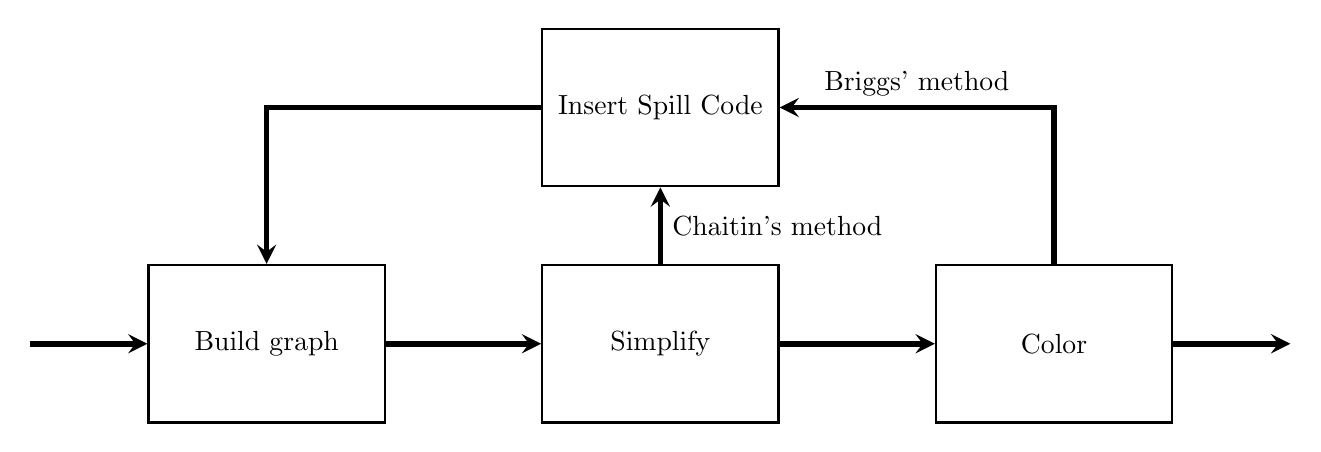
\begin{tikzpicture}[auto,
			    box/.style={inner sep=0mm,minimum height=2cm,minimum width=3cm,draw},thick,
			    edge/.style={->,>=stealth,line width=2pt},
			]
	    \node[box] (build) at (0,0) {Build graph};
	    \node[box] (simplify) at (5,0) {Simplify};
	    \node[box] (color) at (10,0) {Color};
	    \node[box] (spill) at (5,3) {Insert Spill Code};
	    
	    %start
	    \draw [edge,->] (-3,0) -- (build.west);

	    %loop
	    \draw [edge,->] (build.east) -- (simplify.west);
	    \draw [edge,->] (simplify.east) -- (color.west);
	    \draw [edge,->] (simplify) -- node [swap] {Chaitin's method} (spill);
	    \draw [edge,->] (color) -- (10,3) -- node [swap] {Briggs' method} (spill.east);
	    \draw [edge,->] (spill.west) -- (0,3) -- (build);

	    %end
	    \draw [edge,->] (color) -- (13,0);
	\end{tikzpicture}
	\caption{Register allocation phases of Briggs and Chaitin \cite{briggs}.}
        \label{chaitin-briggs}
	\end{figure}

\subsection{Chow Hennesy}
Chow-Hennesy assume that all variables reside in memory and are loaded into registers as required. This is the reverse concept of
Chaitin and Briggs. A priority function is used to calculate the saving when a variables is kept in a register 
instead of the memory. The variables which have the greatest savings are then selected to be stored in registers. Chow-Hennesy's
register allocator works on procedure level.

If no suitable register is found, then live range splitting is applied.\\

Steps in the Chow-Hennesy algorithm:
\begin{enumerate}
 \item Separate the \textbf{unconstrained live ranges} and handle to handle them in the last step. Unconstrained live ranges are those 
       which have less neighbours than available registers.
 \item Repeat steps a) to c), each time assigning a color to a live range until all constraint live ranges have been assigned a color or
       until there is no register left that can be assigned to any live range in any basic block.
 \begin{enumerate}
  \item Compute the priority function $P(lr)$ for each constraint live-range lr if has not been computed. If $P(lr)$ is negative, or if 
        $lr$ is uncolorable, mark $lr$ as a noncandidate, and leave it unassigned. Delete $lr$ from the interference graph.
  \item Find the live range with the highest priority function, $lr*$, and assign a color to it. The color must not be in the
        \textbf{forbidden} set for $lr*$. The forbidden set lists registers that are not allowed as target registers for the given live 
        range. For each live range that $lr*$ interferes with, update the \textbf{forbidden} information.
  \item Check each live range interfering with $lr*$ to see if it needs to be split. A live range needs to be split if all of its target 
        registers are in its forbidden set.
 \end{enumerate}
 \item Assign colors to the unconstrained live ranges, each time choosing a color not belonging to their forbidden set.
\end{enumerate}

\paragraph{Priority function:} The priority function $P(lr)$ assigns a priority to each live range $lr$ to determine if it should be 
allocated to a register. $P(lr)$ is computed as the sum of execution time savings divided by the number of units in each live range:
\begin{align}
 S(lr) &= \sum_{i\in lr}{s_i \times w_i}\\
 P(lr) &= \frac{S(lr)}{N}
\end{align}
with
\begin{itemize}
 \item $s_i$ = Weighted sum of load costs, store costs and move costs per unit. A unit is normally a basic block.
 \item $w_i$ = Estimated execution frequency
 \item $N$ = Number of live units in the live range
\end{itemize}

\paragraph{Live range splitting:} If a symbolic register has a very long live range it can be split into two parts, this way each smaller 
live range can be spilled separately if necessary. Live range splitting can be easily added to Chaitin and Briggs but was not present in 
the original algorithms.

\subsection{Differences and related concepts}
Besides knowing the algorithms, it is important to know some of their differences. The following differences between the algorithms have 
been emphasised in the lecture. Additional differences can be found in the paper of Chow-Hennesy, which contains a summary of the 
differences between Chaitin and Chow-Hennesy's algorithms (see \cite{chowhennesy}, Section 6).

\begin{itemize}
 \item Both Chaitin and Briggs algorithms need multiple iterations where as Chow-Hennesy finishes in one iteration. The reason is that
       for Chaitin and Briggs the insertion of spill code may block additional registers thus requiring more live ranges to be spilled 
       (see Figure \ref{chaitin-briggs}).
 \item Chaiting and Briggs do the life range analysis on instruction level where as Chow-Hennesy perform life range analysis 
       on basic block level. This is because Chaitin and Briggs do register allocation after instruction selection, but Chow-Hennesy's 
       algorithm works on the intermediate code level.
 \item Chaitin and Briggs do register allocation for all registers, where as Chow-Hennesy only do register allocation outside of basic 
       blocks.
\end{itemize}

The following paragraph summarizes some concepts that are relevant in connection with register allocation.

\paragraph{Calling conventions:} Calling conventions are conventions about how registeres are used and who is responsible to save and 
restore them. There are \textbf{caller-saves} and \textbf{callee-saves} registers. The conventions are a result of a multi-step 
proceedure. First the architecture has an impact on the calling conventions, then the operating system and lastly the used programming 
language. Calling conventions are part of the ABI and if not taken care of they my cause incomparibilities between programm binaries such 
as if libraries are used or programms written in different languages interact.

\paragraph{Pre-coloring:} Pre-coloring is used to assign correct colors to argument registers to avoid unnecessary copy instructions.

\paragraph{Rematerialization:} Some optimizations in Section\, \ref{sec:optimization}\, such as \textit{common subexpression
elemination} optimize a program by removing redundant computation. The disadvantage of such an optimization can the that more symbolic 
registers are used or that the live range of a symbolic register is increased. However sometimes it can be cheaper to recompute a value 
than to store it in a register. This is often the case if a value can be recomputed with a single instruction. Rematerialization 
recomputes a value from another value such that instead of two values only one value needs to remain in a register and the other can be 
recomputed when needed. Rematerialization is often used in address calculation such as adding a constant value to an address. For example 
in \lstinline|*p = *q + 2;|, if $p$ is used at different locations in a function it can either remain in a register or be recomputed
from $q$ each time it is needed. Rematerialization is commonly done by register allocators when it is easier to recompute a value, than
to keep it in its own register or to reload it from memory.

\section{Coallescing}
Coallescing is a form of copy elemination that finds registers that are copies of each other and removes the copy instruction, thus
putting the values into the same register. Coallescing may affect the colorability of an interference graph (both negative and positive
results are possible).
\begin{itemize}
 \item Aggressive coallescing (used by Chaitin): Remove all possible copy instructions, may result in increased spilling.
 \item Conservative coallescing: Performs coallescing only when graph colorability is not affected. Was intended to be an improvement but 
       later analysis showed that the algorithm actually performed worse than aggressive coallescing.
 \item Iterative coallescing: Eliminates more copies by interleaving conservative coallescing with simplification phases (like Briggs). 
       Also has worse results than aggressive coallescing.
 \item Optimistic coallescing: Aggressive coallescing, but the algorithm memorizes what has been coallesced. If coloring is not possbile 
       and nodes need to be spilled, then the coallscing is reversed by live range splitting and then only parts of the nodes are spilled 
       if possible. \textbf{Best results}.
\end{itemize}

\section{Optimal register allocation using integer linear programming}
Performance overhead of spill code is minimized by using integer linear programming to achieve near optimal results. Since the problem is 
NP-complete an optimal solution will be instractable for very complex problems. However the Optimal Register Allocator (ORA) solver still 
produces very good results that are very often within 1\% of the optimal solution. However in order to define what optimal means we need 
to know which optimizations are being done (or not done) by the register allocator.\\

\noindent \textbf{What does the register allocator do and not do?}
\begin{enumerate}
 \item The register allocator does not reorder instructions.
 \item The register allocator adds only spill load instrucitons, spill store instrucitons, and rematerialization instructions.
 \item The register allocator removes only copy instructions and instructions defining symbolic registers that are rematerialized.
 \item All controll-flow paths throguh a function can potentially execute.
 \item At a given location, the cost of a spill instruction is a fixed number of cycles (based on the instrucitons' type) times the 
       location's estimated execution count.
 \item A basic block's estimated execution conut equals the sum of the countes exeiting the block, i.e. estimated execution counts 
       satisfy Kirchhoff's current law over the control flow graph.
\end{enumerate}

The ORA implementation is composed out of three modules. The analysis module analyzes a functions control flow graph and identifies 
points which require a decision about register allocation actions. For each decision a boolean decision variable is introduced that 
records if the decision is made (1) or not (0) and also what action is taken if the variable is set to 1. These decision variables are 
then build into a series of \textbf{inequalities} that model constraints for the decision variables. The solver module then solves these 
inequalities and finally the rewrite module rewrites the code according to the results in the decision variables.

\subsection{ORA Modules}
Most of the paper focuses on the \textbf{analysis module} and explains the steps to derive (in)equalities from decision variables. The 
steps in the analysis module are as follows:

\begin{itemize}
 \item Use live range analysis on the functions control flow graph and build an \textbf{instruction graph} for each symbolic register. 
       The instruction graph contains solid and dashed lines for each symbolic register to show active and inactive live ranges, 
       respectively.
 \item Apply transformations to create a \textbf{symbolic register graph}. Each transformation can potentially create one or more
       conditions. A \textbf{condition} is an equality or inequality function containing decision variables to constrain the valid 
       assigments to the decision variables. The following gives an example for such a condition: 
       \begin{align}
        x_{defA} &= x_{use-end1A} + x_{use-cont1A}
       \end{align}
       This condition ensures that if the symbolic register $A$ is allocated to a register at the given instruction, then its use must 
       either end at that point or it must continue. At this point decision variables are not yet tied to real registers, that happens
       in the next step.
 \item A copy of each symbolic register graph and its associated set of conditions is made for each \textbf{real register} that is
       available for allocation. For example:
       \begin{align}
        x^1_{defA} + x^2_{defA} &= 1
       \end{align}
       This condition requires that the symbolic register $A$ is allocated to exactly one physical register, either register $1$ or 
       register $2$, but not to both or none.
 \item Next several additional conditions are added to ensure that the solution is correct and optimal. For example conditions are 
       added such that not too many or too few symbolic registers are allocated to real registers, or to ensure optimal spill code 
       placement.
 \item Another additional transformation is for rematerialization. If a symbolic register can be rematerialized (see Section 
       \ref{sec:register-allocation}), then the register allocator adds conditions to allow rematerialization instead of spilling
       and loading a symbolic register.
\end{itemize}

When all conditions have been created they are passed to the solver module to find a valid solution for all decision variables.

\subsection{Results}
The experimental results show that the ORA performs significantly better than other register allocators and is able to remove many
copy instructions and reduce the overhead of spill code significantly. There exists a second paper that was written six years later and 
discusses improvements to the original ORA implementation. The authors were able to reduce the complexity of the algorithm 
from $n^3$ to $n^{2.5}$. They also improved the speed by a factor of 1000x (10x CPU, 10x better solver, 10x improved model).


\section{Interproceedural register allocation}
Interproceedural register allocation (which is also often called global register allocation) performs register allocation accross
proceedures or compilation units and not just within a single function as is done in global register allocation. This solves the problem
that different functions may assign the same global variable to different registers or the same register to different local variables, 
which causes unnecessary copy instructions.

\subsection{Global Register allocation at link time (Annotation based)}
Global here means interproceedural accross all compilation units. The register allocation is split into three parts:
\begin{itemize}
 \item Compiler
 \item Register allocator
 \item Linker
\end{itemize}
The compiler does as much work as posible in order to maximize the benefits of seperate compilation such that in the linking phase there 
is not too much work required. The compiler inserts annotations into the object code which describe how variables are used. Annotations 
provide information to the linker about how to replace variables and how to rewrite the code. The following six annotations are inserted 
by the compiler. Each annotation is tied to a variable $v$. When the linker is run, it analyses the object code to identify if $v$ has 
been assigned to a register. If $v$ is in a register then the corresponding action is appied, otherwise the annotation is ignored.

\begin{itemize}
 \item \makebox[4.3cm]{REMOVE.v\hfill} Remove the instruction
 \item \makebox[4.3cm]{STORE.v\hfill}  Replace store by copy instruction 
 \item \makebox[4.3cm]{LOAD.v\hfill}   Replace load by copy instruction
 \item \makebox[4.3cm]{OP1.v, OP2.v, RESULT.v\hfill} Replace operands or result by register
\end{itemize}

The register allocator generates a call graph and uses the information provided by the compiler assign variables to registers. It does 
this by building groups of variables that are not active at the same time and then assigns a usage frequency to those groups. The same 
happens for global variables. Finally the groups with the highest freuqencies are allocated to registers. After variables have been 
assigned to registers the linker can use this information rewrite the code and to apply the actions that have been stored in the 
annotations. While doing this it must take care to adjust addresses of instructions or data if a previous instruction is being removed.

Additional considerations concern initialization and recursion.

\subsubsection*{Initialization}
Special care must be taken to initialize global variables and proceedure parameters. For global variables an INIT action is placed at the
beginning of the program and runs when the program is invoked. The INIT action contains instructions to copy the initial value of global 
variables from memory to the respective register.

\subsubsection*{Recursion and indirect calls}
Recursion means that the same proceedure my be called repeatedly befor the first invokation has been completed. Therefore the program
needs to take care to save the necessary registers of local variables before the next invokation of the proceedure. The question is who 
should be responsible to save the local varibles of the proceedure. It turns out that it is not enough if each recursive proceedure is 
responsible to save its local variables because this would not archive local variables of other proceedures in the call chain. The 
solution is to let the proceedure that makes the recursive call save the local variables of all proceedures in the call chain. The same 
solution is used for indirect calls.

\subsection{Register allocation across procedure and module bounaries (Web)}
This has two important parts, the web algorithm itself and clustering (e.g. spill code motion).
\subsubsection*{Web algorithm:}
Performs several steps:
\begin{enumerate}
 \item Reads in source files and produces intermediate representation files.
 \item Creates program database.
 \item Uses Program database and transforms intermediate representation files into object files.
 \item Linking of the object files.
\end{enumerate}
The web algorithms creates a table with L\_REF, P\_REF, and C\_REF entries from which a web interference graph is generated. This is then
used to apply a coloring on the graph that determines which register is being used for each global variable.

\subsubsection*{Clustering (Splill code motion):}
The idea is to move spill code for callee-saved registers inside a cluster from one node to
its dominating node. If the node is being called more than once, then the overhead of the spill code is reduced. Same for caller-saved 
registers which are moved down to lower nodes in the same cluster.

\section{Instruction Scheduling}
Instruction scheduling is an optimization that deals with rearranging the instructions of a program to better exploit the inherent
parallelism of the instructions. The goal is to move instructions that depend on each other further appart and instead insert independent
instructions inbetween. This prevents that dependent instructions block the processor pipeline and allows a more instructions to execute 
simultaneously. The simplest form of instruction scheduling is called list scheduling because from a list of possible instruction that 
can be scheduled one with the highest priority is selected based on some kind of heuristic. There exist two papers that deal with list
scheduling which both present different heuristics for the problem. The list scheduling algorithms presented in the papers have a worst 
case complexity of $O(n^2)$ needed to build the dependency graph. However in practice there exists also a linear time algorithm.

The improved \textbf{linear time algorithm} works as follows. The algorithms goes through each instruction and each time a register is 
defined the algorithm saves which instruction defined the register. Each time a register is accessed the corresponding instruction can be 
looked up and the algorithm adds a dependency to the graph. The only problem with this algorithm is that the initialization of the 
corresponding data structure may be expensive. However this can be optimized when using virtual registers by storing from which 
instruction to which instruction a basic block extends. Based on these limits it can be easily determined if an instruction is still 
independent. Otherwise the datastructures would need to be rebuild for each basic block.

\subsection{Phase ordering problem:}
A problem between instruction scheduling and register allocation is that both optimizations can have negative effects on the other one, 
thus it is difficult to decide what should be done first -- register allocation or instruction selection. This problem is called the
\textit{phase ordering problem}. The list scheduling algorithms below attempt different solutions but still perform both optimizations 
separately. A better solution is discussed in the next Section which presents algorithms that perform instruction scheduling and register
allocation together at the same time.

The impact of each optimization to the other is as follows:
\begin{itemize}
 \item Register allocation serializes the code and removes opportunities for scheduling (less instruction level parallelism).
 \item Instruction scheduling increases the length of the live ranges (register pressure), causing more interferences and thus requires 
       the use of more registers or increased spilling.
\end{itemize}

\subsection{Instruction scheduling for the IBM RISC System/6000 Processor (IBM)}
The algorithm which is described in this paper performs the instruction scheduling twice, once before register allocation and once
afterwards. The first instruction scheduling has more freedom since register allocation has not yet been done, but register allocation
may insert spill code and delete move instruction which make a second run of instruction scheduling necessary. The algorithm itself works
as follows:
\begin{itemize}
 \item It uses a dependency graph which is constructed for each basic block. The dependency graph has one node for each instruction and
       adds a directed edge between two instructions if one needs to preceed the other.
 \item Edges are labeled with the delay between instructions.
 \item After the dependency graph has been build, nodes are labled upwards with the \textbf{maximum delay} from the node to the end of 
       the basic block (red digits in Figure \ref{dependency-graph}).
 \item The algorithm keeps a \textbf{current time} counter, which is initially zero. It is increased by the execution time of each 
       scheduled instruction, which is usually one.
 \item Nodes are labels with \textbf{earliest time} value which is calculated from the current time of the last scheduled predecessor 
       plus the delay of that instruction to its successor. For example the node L.B has a delay of one and is scheduled in step 2 where 
       the current time is increased to 2, so the ADD node would be labled with an earlies time of 3 (2+1).
\end{itemize}

Figure \ref{dependency-graph} shows the the dependency graph from the paper but adds the values of the maximum delay and a table that 
shows how the current time is updated and which instruction is selected in each step.

\begin{figure}[h!]
\begin{tikzpicture}[node/.style={circle, draw, thick, minimum size=1.0cm,inner sep=0pt,font=\footnotesize,align=center},
		    item/.style={inner sep=0pt,font=\footnotesize,align=left},
		    edge/.style={->,>=stealth,line width=2pt},auto,
		    red/.style={draw=red},black/.style={draw=black},
		    legend/.style={draw=black}
		   ]
    \node[node]  (la) at 	(1, 7) {L.B 	\\ \textcolor{red}{1}};
    \node[node]  (lc) at 	(3, 7) {L.C 	\\ \textcolor{red}{1}};
    \node[node]  (ld) at 	(4, 5) {L.D 	\\ \textcolor{red}{1}};
    \node[node]  (le) at 	(8, 3) {L.E 	\\ \textcolor{red}{4}};
    \node[node]  (add) at 	(2, 5) {ADD 	\\ \textcolor{red}{0}};
    \node[node]  (sub) at 	(3, 3) {SUB 	\\ \textcolor{red}{0}};
    \node[node]  (store) at 	(4, 1) {ST.A 	\\ \textcolor{red}{0}};
    \node[node]  (compare) at 	(8, 1) {CMP	\\ \textcolor{red}{3}};
    \node[node]  (branch) at 	(6, 0) {BC	\\ \textcolor{red}{0}};

    \draw[edge]  (la)      -- node [swap] {1} (add);
    \draw[edge]  (lc)      -- node        {1} (add);

    \draw[edge]  (ld)      -- node        {1} (sub);
    \draw[edge]  (add)     -- node [swap] {0} (sub);

    \draw[edge]  (sub)     -- node        {0} (store);
    \draw[edge]  (store)   -- node        {0} (branch);

    \draw[edge]  (le)      -- node {1} (compare);
    \draw[edge]  (compare) -- node {3} (branch);

    \node[legend] (foo) at (11,6) {
	\begin{tikzpicture}
	    \node[item] (step1) at (0,  0) {1. Current time: $0\rightarrow1$;\quad select L.E\\
					    2. Current time: $1\rightarrow2$;\quad select L.B\\
					    3. Current time: $2\rightarrow3$;\quad select CMP\\
					    4. Current time: $3\rightarrow4$;\quad select L.C\\
					    5. Current time: $4\rightarrow5$;\quad select L.D\\
					    6. Current time: $5\rightarrow6$;\quad select ADD\\
					    7. Current time: $6\rightarrow7$;\quad select SUB\\
					    8. Current time: $7\rightarrow8$;\quad select ST.A\\
					    9. Current time: $8\rightarrow9$;\quad select BC};
	\end{tikzpicture}
    };

    \node[legend] (foo) {
	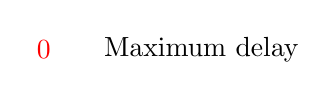
\begin{tikzpicture}
	    \node (redsquare) at (-2, -1) {\textcolor{red}{0}};
	    \node (redlegend) at (0, -1) {Maximum delay};
	\end{tikzpicture}
    };
\end{tikzpicture}
\caption{Dependency graph constructed by IBM instruction scheduling algorithm}
\label{dependency-graph}
\end{figure}

When deciding which node to select in each step, the algorithm uses an eight step heuristic. Since there is no planning or lookahead 
involved the algorithm is not guaranteed find the best solution. There are the following seven heuristics:
\begin{enumerate}
    \item Initialize the set of all those instructions that have not yet been selected, and that have no predecessors in the dependency 
          graph (these are the ''legal`` ones).
    \item Refine the subset to those instructions whose earliest time has arrived or, if none, those with the smallest earliest time.
    \item If one or more instructions have been selected, and if the current subset contains one or more instructions of opposite type 
	  (fixed/floating) from the last one selected, then refine the current subset to those of this opposite type.
    \item Refine the subset to those of maximum total delay along the path of each instruction to the end of the basic block.
    \item Refine the subset to those of minimum ''liveness weight``.
    \item Refine the subset to those with greatest uncovering''.
    \item Refine the subset to the unique instruction that came first in the original ordering.
\end{enumerate}

\subsection{Efficient Instruction Scheduling for a Pipelined Architecture (HP)}
The general idea is similar to the IBM algorithm. The algorithm works as follows:
\begin{enumerate}
 \item Build a scheduling dag over the basic block
 \item Put the roots of the dag into a candidate set
 \item Select the first instruction to be scheduled based on the heuristics below
 \item While the candidate set is not empty do the following:
    \begin{enumerate}
    \item based on the last instruction scheduled and the heuristics select and emit the next instruction that should be scheduled
    \item delete the instruction from the dag and add any newly exposed candiates
    \end{enumerate}
\end{enumerate}

The following heuristics use the following criteria to determine the priority with which a candidate should be scheduled:
\begin{enumerate}
 \item Whether an instruction interlocks with any of its immediate successors in the dag.
 \item The Number of the immediate successors of the instruction
 \item The length of the longest path from the instructions to the leaves of the dag.
\end{enumerate}

The instruction scheduling in is performed before register allocation. The paper mentions register allocation but claims that 
''serializing definitions does not unduly restrict [the] code``.

\section{Register allocation \& instruction scheduling}
This section introduces three methods which combine instruction scheduling and register allocation in order to solve the phase
ordering problem. The first paper presents two algorithms the Integrated Prepass Scheduling (IPS) and the dag-driven register allocation.
The second paper introduces a method named Register Allocation with Scheduling Estimate (RASE).

\subsection{Integrated Prepass Scheduling}
The main issue of the phase ordering problem is that register allocation reduces opportunities for scheduling while instruction scheduling 
increases the length of live range making register allocation more difficult. The IPS algorith solves this problem by using two strategies 
that can be selected depending on what strategy is more appropriate. The two strategies are:
\begin{itemize}
 \item CSP (Code scheduling for pipelined processors) reduces pipeline delays but can increase the lifetime of registers. It is used if 
       enough free registers are available.
 \item CSR (Code scheduling to minimizes register usage) is used when the number of registers is low to control register usage. It tries
to ''find the next instruction which will not increase the number of live register or if possible, decrease that number``.
\end{itemize}
IPS uses a simple heuristic to switch between the two strategies, it keeps track of the number of available registers in a variable named 
AVLREG, if the number of free registers drops below a certain threshold, then it switches to CSR. When AVLREG has increased above the 
threshold then it switches back to CSP.

\subsection{Dag-driven register allocation}
Dag-driven register allocation is a form of postpass scheduling to keep the graph flat and wide. It also does not insert any 
additional spilling instructions into the code. The algorithm introduces two measures for the graph the width and the height:
\begin{itemize}
 \item The \textbf{width} is defines as the maximum number of mutually independent nodes. Wider graphs indicate higher parallelism.
 \item The \textbf{height} is the length of the longest path. If the graph is too high then code scheduling becomes less efficient.
\end{itemize}
The goal of the dag-driven register allocator is to balance the dag. To do that it will \textbf{minimize the height} of the graph and 
\textbf{limit the width} of the graph to a number that is less or equal to to the amount of registers available.

The dag-driven register allocator uses two techniques to achieve these goals:
 \begin{itemize}
  \item First, it makes use of free WAR dependencies. That is, it makes use of redundant dependencies when allocating registers. Such 
        redundant dependencies can occur for example if a RAW dependency already exists between two instructions. In the Listing below 
        assume registers \lstinline|R2| and \lstinline|R4| are available for reuse in the second instruction. There is already a RAW 
        dependency for \lstinline|R5|, so when register \lstinline|R4| is choosen a redundant WAR dependency is added. This WAR 
        dependency is free because of the existing RAW dependency for \lstinline|R5|, so \lstinline|R4| is a better choice than 
        \lstinline|R2|. When reusing registers, the dag driven register allocator will prefer those registers that only introduce redundant dependencies. 


\begin{lstlisting}[xleftmargin=3.5mm]
Add R5, R4, R1
Sub ??, R5, #4
\end{lstlisting}

  \item Second, it tries to balance the growth of the dag. When a register is reused and the register allocator cannot make use of a
        free WAR dependency then it must add a dependency which connects two independent paths and the height of the dag will be 
        increased. So the important part in balancing the dag is to find a path to connect the path of the current instruction, such that 
        it does not increase height of the dag too much. To achieve this for each instruction the \textit{earliest issue time (EIT)} and 
        \textit{earliest finish time (EFT)} are computed. The register allocator now tries to find two paths such that one has a high
        EIT and the other has a large EFT.
 \end{itemize}

\subsection{Register Allocation with Scheduling Estimate (RASE)}
The RASE approach is an integrated scheduling and register allocation method. The idea behind RASE is to perform a pre-scheduling in 
order to calculate schedule cost estimates that enable the register allocator to make a decision about how many registers it is going to 
use. Essentially RASE splits the available registers into two parts, one part for the register allocator, and one part for the 
instruction scheduler. The RASE algorithm has three phases:

\begin{enumerate}
 \item Pre-scheduling
 \item Global register allocation
 \item Instruction scheduling with local register allocation
\end{enumerate}

The \textbf{first phase} is the pre-scheduling, which calculates the schedule cost estimate. During the pre-scheduling, the order of the 
instructions is not changed.

The \textbf{second phase} performs a \textit{global} register allocation using the schedule cost estimate, but leaves enough free 
registers for the last phase. The schedule cost estimate allows the register allocator to estimate, how the cost of local register 
allocation increases, if it uses more registers to allocate \textit{global} symbolic registers. In the second phase the register 
allocator is only responsible for allocating global symbolic registers to physical registers, the allocation of \textit{local} symbolic 
registers is defered until the third phase.

The \textbf{third phase} performs the instruction scheduling and does the \textit{local} register allocation.  This register allocation 
must be within the limits for \textit{local} registers that have been determined in the second phase.

\textbf{How does the schedule cost estimate function work?} The schedule cost estimate is a quadratic function (of \textit{regressive} 
form). It takes as input the number of local registers and returns as output the estimated machine cycles:
\begin{figure}[h!]
\begin{center}
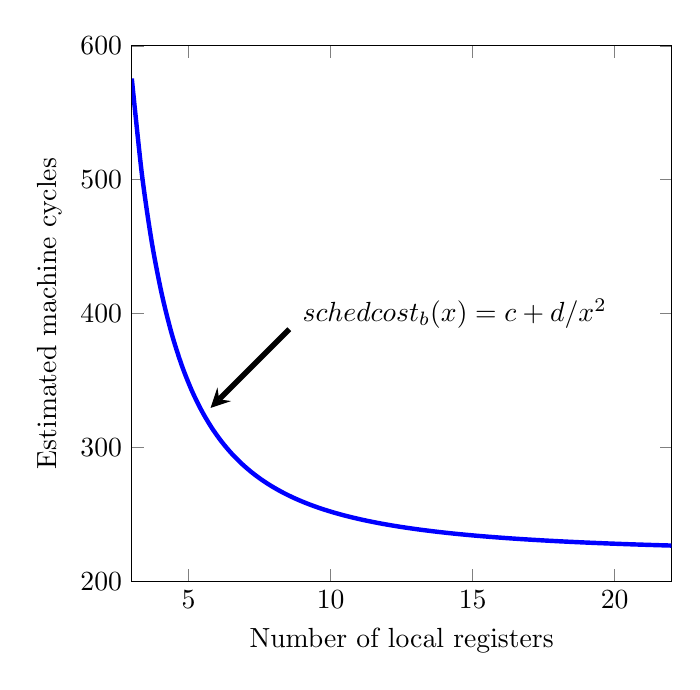
\begin{tikzpicture}
   %\draw[->] (-0.5,0) -- (4.2,0) node[right] {$x$};
   %\draw[->] (0,-0.5) -- (0,4.2) node[above] {$y$};

    \begin{axis}[xmin=3,xmax=22,ymin=200,ymax=600,samples=55,y=0.017cm,
                 xlabel={Number of local registers},
                 ylabel={Estimated machine cycles}]
     \addplot[blue, smooth, ultra thick, domain=3:22] (x,{220+3200/(x*x)});
    \end{axis}

   %\draw[scale=0.5,domain=1:8,smooth,variable=\x,blue] plot ({\x},{1 + (7 / \x^2)});
   \draw[<-,>=stealth,line width=2pt] (1,2.2) -- (2,3.2) {};
   \node (formula) at (4.1,3.4) {$schedcost_b(x)=c+d/{x^2}$};
\end{tikzpicture}
\end{center}
\caption{Schedule cost estimate function}
\label{schedule-cost-estimate-function}
\end{figure}

The coefficientes $c$ and $d$ are computed as part of the pre-scheduling. Essentially this function allows the register allocator to 
estimate how much the required machine cycles are incresed, due to loss of parallelism, if the available local registers are reduced.
As can be seen in Figure \ref{schedule-cost-estimate-function}, if the register allocator leaves 15 registers to the third phase,
then the total execution cost for that basic block it not very high, however if only 4 or 5 registers are left to the third phase,
then the cost increases quite significantly.

\subsection{Which algorithm should be prefered?}
When comparing the three algorithms one can say that IPS is the ''best`` 
algorithm, because it is realively easy to implement and produces results which are comparable to the other two solutions. The IPS 
algorithms can be easily implemented in existing register allocators such as Chaitin or Briggs. In contrast the DAG driven algorithm and 
RASE are both quite complicated to implement but do not produce significantly better results.

\section{Trace scheduling}
Trace scheduling attempts to provide another solution for the phase ordering problem. A trace is \textbf{a sequence of instructions that 
can have exit and entry points but that must not have any loops}. The trace 
scheduler orders traces by their frequency and schedules the most frequent trace first. Inner most loops usually contain 
the traces with the highest frequency and are thus scheduled first. Since the instruction scheduler is also responsible for assigning 
variables to registers, this scheduling approach effectively gives priority to those variables, which are used with the highest frequency.
The advantage of this approach is that at the beginning all registers are available for use by the scheduler, giving the scheduler 
complete choice over registers with the highest frequency.

Since traces are scheduled individually of each other care must be taken if two traces merge with each other or split from each other.
This can either happen at split nodes, when one trace leaves from the other, or at join nodes, when one trace joins into another. Since 
the traces are scheduled and register allocated individually there needs to be a machanism to communicate register allocation decisions
between traces. This is done by adding special nodes named \textit{Value Location Mapping} (VLM).

\subsection{Variable Location Mapping (VLM):} 
A VLM is placed at the split or join nodes between two traces and contains the information about already allocated variables. So when a 
trace is scheduled that contains a variable which has already been allocated, then the scheduler can take this decision into account. It 
tries to ensure that individually scheduled traces reference their values at the same locations to avoid unnecessary data motions such as 
register moves, spills and restores. If a VLM appears at the beginning of a trace, then the scheduler must make sure to read values that 
appear in the trace from the locations specified in the VLM. On the other hand, if a VLM appears at the end of a trace, then the 
scheduler must make sure to \textit{satisfy} the references in the VLM, that is, it must store values that appear in the trace at the 
locations specified by the VLM. Sometimes it may not be possible to satisfy the constraints in a VLM. This can happen if there is a VLM 
both at the top and bottom of a trace and both VLMs have conflicting locations for the same variable. If it is not possible to satisfy 
the location constraints in a VLM, then the scheduler must insert \textbf{compensation code} to move or copy values to the correct 
locations.

\subsection{Delayed binding}
Delayed binding is used because some values have live ranges that go through a trace but the value is not actually used inside the 
trace. \textit{''A delayed binding is a sort of pseudo-location that may be assigned to an unreferenced value by the instruction 
scheduler.''} Delaying the variable binding until there is an actual reference to it helps to preserve registers for more important 
values. When a delayed binding is bound to an actual location it is determined if there exists an unused register that is free through out 
the whole live range of the value, otherwise the value is bound to memory.

\textbf{Paper Evaluation:} The evaluation of the trace scheduling paper is not useful, because the results are only compared to 
themselves.

\section{Software pipelining}
Software pipelining is a form of instruction scheduling with the goal of scheduling the different instructions of a loop in a way, such 
that multiple loop iterations can be active at the same time.

\subsection{Modulo Variable Expansion}
One problem in software pipelining is that a variable is defined and then used two cycles later. If 
this variable remains in the same register during every loop iteration, then each iteration must take two cycles. However if copies of 
the variable are kept in different registers for consequtive iterations, then it is possible to start a new operation in each cycle.
This concept of using multiple registers for the same variable is called \textbf{modulo variable expansion}.

%TODO: Which problems occur du? What is it? Why is it needed?

\subsection{Resource-constrained software pipelining}
This algorithm provides a solution to the software pipelining problem by combining instructions into sets of available instruction which 
are then scheduled. The algorithm is very elegant but has the grave problem that the algorithm is only shown graphically, the actual
\textbf{heuristic} to choose which instructions can be combinede into the sets and how to schedule them \textbf{is missing} and thus the 
algorithm cannot be implemented.

\subsection{Iterative modulo scheduling:}
Different scheduling strategies exist in software pipelining, the iterative modulo scheduling is a form of the ``schedule-then-move''
stategy. The goal of iterative modulo scheduling is to find a schedule for the instructions of a loop body, such that the loop
can be repeated at regular intervals, without causing any conflicts between the instructions. There are two types of conflicts that can
occur, a resource conflict or a dependency conflict:
\begin{itemize}
 \item Resource conflict: The same processor resource such a bus or a pipeline stage are in use at the same time.
 \item Dependency conflict: Can be an inter-iteration-dependency if there exists a dependency between instructions in two different 
       iterations of a loop or an intra-iteration-dependency if there is a dependency between two instruction in the same loop iteration.
\end{itemize}
Before the actual iterativev modulo scheduling is performed several other optimizations and transformations are performed, one of them is
IF-conversion. \textbf{IF-conversion} removes all branches except the loop closing branch and converts the code into a single basic block. The different branches of the original code are instead expressed by data dependencies involving predicates.

Iterative modulo scheduling introduces the notion of an \textbf{initiation intervals (II)} which is the interval between the start of a 
new loop iteration. An II of four means that every 4-th instruction a now loop iteration begins. A \textbf{minimum initiation interval 
(MII)} is calculated and used to calculate the minimum length of a schedule. To compute the actual II a 
candidate II is used that is initialy set to the MII and then step wise incremented until a suitable II is found. The MII is the maximum 
of the Resource constraint MII and Recurrence constraint MII values:

\begin{itemize}
 \item The \textbf{Resource-constrained MII} used to avoid that two instructions block the same processor resource at the same time. For 
       example if an add instruction requires to use the result bus in the fourth cycle and a multiply instruction requires the result bus 
       in the sixth cycle, then an add cannot be sheduled two cycles after a multiply. The ResMII can be computed by performing a
       bin-packing of the reservation tables for all the operations.
 \item The \textbf{Recurrence-constrained MII} is used prevent data dependencies between the same operations in different loop iterations. 
       % TODO: How does this work?
\end{itemize}

The iterativ modulo scheduling starts with the initially computed II and tries to find a valid schedule for this II and a given budget. If
no schedule can be found the II is increased by one and the proceedure is repeated until a schedule is found. There are some differences
between the traditional acyclic list scheduling and iterative modulo scheduling:
\begin{itemize}
 \item Instructions can also be unscheduled and rescheduled, thus operation scheduling instead of instruction scheduling is performed. 
       Operation scheduling picks an instruction and scheduls it at a time slot that is both legal and most desirable.
 \item Instructions do not become ``ready'' after their predecessors have been scheduled. Instead the algorithm keeps track of which 
       instructions have never been scheduled and schedules instruction based on a priority function.
 \item If an instruction is unscheduled it is immediately rescheduled.
\end{itemize}

\subsection{Optimizations for processors with SIMD instructions}
Processors with SIMD instructions allow to execute the same sequence of instructions on multiple instances of data such as arrays. For
this purpose the data must be naturally aligned on the block size. If the alignment cannot be statically determined at compile time
then the compiler needs to insert dynamic runtime checks that verify if the pointers are aligned. If the pointers are aligned then
SIMD instructions can be used, otherwise the memory is accessed sequentially. These dynamic checks increase the program size and impact 
the execution speed. Not only the dynamic checks increase program size, but also the fact that there need to be two versions of a loop,
one version with SIMD instruction and another version which accesses memory locations sequentially.

The paper describes an algorithm to generate SIMD instructions for logical and arithmetical operations as well as SIMD load and
store instructions. Further more it describes an analyzation technique to statically identify the alignment of C pointers. 
This alignment information can then be used to reduce dynamic alignment checks and thus reduce the overhead of those checks. 
About 50\% of all pointers can be statically identified.

\subsubsection{SIMD Instruction Generation}
The SIMD instruction generation consists of two phases:
\begin{itemize}
 \item Phase 1 deals with the generation of logical and arithmetical SIMD instruction inside loops that process arrays.
 \item Phase 2 deals with the generation of LOAD and STORE SIMD instructions for data that is used by the logical and arithmetical SIMD 
       instructions which have been generated in phase 1.
\end{itemize}

In order to generate logical and arithmetical SIMD instructions from loops the \textbf{loop must be unrolled $k$ times}, where $k$ 
depends on the number of elements in a SIMD instruction. For example if a loop processes 16bit elements and the SIMD operands are 32bit
then the loop needs to be unrolled two times. If the loop count is not a multiple of $k$ then a pre- or postloop is added which is 
executed $N \mod k$ times, where $k$ is the unroll count and $N$ the loop count. Depending on the alignment information a preloop or
a postloop is added.

The main reason for loop unrolling is get an \textbf{acyclic dependency graph} for the loop body which contains enough equivalent
expressions that can be combined into a SIMD instruction. The nodes in the graph are \textit{s-nodes} (statement nodes) and
\textit{b-nodes} (groups of basic blocks). The algorithm first schedules s-nodes that are not candidates\footnote{Candidates are
those nodes for which SIMD instructions are available on the platform. For example if the target processor does not support a special
SIMD instruction for multiplication then nodes with multiplications are not candidates for SIMD instructions.} for SIMD instructions
as well as all b-nodes. Then it tries to find a series of s-nodes which are structurally equivalent and combines them into a SIMD
instruction. To identify the instructions that can be combined into SIMD nodes, the algorithm builds \textit{``all possible
combinations of SIMD candidates and rates them according to the number of resulting SIMD expressions and the number 
of adjacent subwords in the SIMD expressions''}. Scheduled nodes are removed from the dependency graph and the proceedure is repeated 
until the graph is empty.

The algorithm also applies scalar expansion and accumulator splitting. Scalar expansion replaces a scalar by an array which 
contains copies of the scalar, such that it can be used with SIMD instructions. Accumulator splitting is used in reductions such as 
calculating the sum of an array. The array is split into several smaller arrays for which the sum can be calculated in parallel, the 
results is then a smaller array from which the final result can be computed.

\subsubsection{Alignment analysis}
The alignment analysis is done by \text{abstract interpretation} of the code. For each expression that modifies a pointer the
algorithm stores the possible remainders modulo $k$, where $k$ is the number of bytes in a SIMD instruction (e.g. 4 on 32bit). Doing
so keeps the possible state space small and prevents a state explosion during the abstract interpretation of the code.

The algorithm first performs an intra-proceedural analysis by examining pointers inside proceedures, followed by an inter-proceedural
analysis. When an array is defined or dynamically loaded, then the first element is already aligned correctly, that is the alignment
is zero modulo the block size. This is enforced by the program loader, the compiler and the function family of \lstinline|malloc|
when memory is allocated dynamically. When a pointer is modified for example through pointer arithmetic, the algorithm computes the
possible remainers of the new pointer. For example for a block size of 4 bytes the possible values for the pointer alignment are
\lstinline|{0,1,2,3}|. If the set of alignment information for a pointer contains only the value \lstinline|{0}|, then the pointer
is correctly aligned, if the set contains multiple values it means that that several alignments are possible. This in the next step
this aligment information is propagated accoss proceedure calls by the inter-proceedural analysis.

Based on the alignment information that the algorithm computed, dynamic checks are inserted if necessary.

\newpage
\begin{thebibliography}{9}
\footnotesize
\bibitem{powerpc}
The PowerPC 604 RISC Microprocessor (S.P. Song \& M.D. Denman), 1994

\bibitem{alpha}
Alpha AXP Architecture (R.L. Sites), 1993

\bibitem{intelp6}
Discorvery 6 - Intels Sternenschiff P6 im Detail (G. Schnurer), ct' 4/1995

\bibitem{compileroptimization}
Advanced Compiler Optimizations For Supercomputers (D.A. Padua \& M.J. Wolfe), 1986

\bibitem{convexfortran}
The CONVEX FORTRAN 5.0 Compiler (R. Mercer), 1988

\bibitem{globaloptimizer}
Effectiveness of a Machine-Level, Global Optimizer (M. S. Johnson \& T.C. Miller), 1986

\bibitem{iburg}
Engineering a Simple - Efficient Code Generator Generator (C.W. Fraser, D.R. Hanson, T.A. Proebsting), 1992

\bibitem{beg}
BEG - a Generator for Efficient Back Ends (H. Emmelmann, F-W. Schr\"oer, R. Landwehr), 1989

\bibitem{pbqp-instruction-selection}
Generalized instruction selection using SSA graphs (Andreas Krall et all.), 2006

\bibitem{briggs}
Coloring Heuristics for Register Allocation (P. Briggs, K.D. Cooper, K. Kennedy, L. Torczon), 1989

\bibitem{chaitin}
Register Allocation \& Spilling via Graph Coloring (G.J.Chaitin), 1982

\bibitem{chaitin2}
Register Allocation via Coloring (G.J.Chaitin, M.A. Auslander, A.K. chandra, J. Cocke), 1980

\bibitem{chowhennesy}
The Priority-Based Coloring Approach to Register Allocation (F.C. Chow \& J.L. Hennessy), 1990

\bibitem{coallescing}
Optimistic Register Coalescing (J. Park \& S-M. Moon), 1998

\bibitem{optimalregisterallocation}
Optimal and Near-optimal Global Register Allocation Using 0-1 Integer Programming (D.W. Goodwin \& K.D. Wilken), 1996

\bibitem{fasterora}
A Faster Optimal Register Allocator (C. Fu \& K. Wilken), 2002

\bibitem{annotations}
Global Register Allocation at Link Time (D.W. Wall), 1986

\bibitem{web}
Register Allocation Across Proceedure and Module Boundaries (V. Santhanam \& D. Odnert), 1990

\bibitem{instructionschedulingibm}
Instruction scheduling for the IBM RISC System/6000 processor (H.S.Warren), 1990

\bibitem{instructionschedulinghp}
Efficient Instruction Scheduling for a Pipelined Architecture (P.B. Gibbons, S.S. Muchnick), 1986

\bibitem{ips}
Code Scheduling and Register Allocation in Large Basic Blocks (J.R. Goodman \& W-C. Hsu), 1988

\bibitem{rase}
Integrating Register Allocation and Instruction Scheduling for RISCs (D.G. Bradlee, S.J.Eggers, R.R. Henry), 1991

\bibitem{tracescheduling}
Phase Ordering of Register Allocation and Instruction Scheduling (S.M. Freudenberger \& J.C. Ruttenberg), 1991

\bibitem{modulovariableexpansion}
Software Pipelining: An Effective Scheduling Technique for VLIW Machines (M. Lam), 1988

\bibitem{realisticsoftwarepipelining}
A Realistic Resource-Constrained Software Pipelining Algorithm (A. Aiken, A. Nicolau), 1990

\bibitem{moduloscheduling}
Iterative Modulo Scheduling: An Algorithm For Software Pipelining Loops (B.R Rau), 1994

\bibitem{simd}
Compiler optimizations for processors with SIMD instructions (I. Pryanishnikov, A. Krall, N. Horspool), 2006

\end{thebibliography}

\end{document}
